
%%%%%%%%%%%%%%%%%%%%%%%%%%%%%%%%%%%%%%%%%%%%%%%%%%%%%%%%%%%%%%%%%%%%%%
%%                     Consumption
%%%%%%%%%%%%%%%%%%%%%%%%%%%%%%%%%%%%%%%%%%%%%%%%%%%%%%%%%%%%%%%%%%%%%%

\subsection{Glyph: \glyph{Consumption}}
\label{sec:consumption}

\glyph{Consumption} is the arc used to represent the fact that an entity pool is consumed by a process, but is not produced by the process. A \glyph{consumption} is represented by a simple line without particular symbols at its extremities. A cardinality label may be associated with \glyph{consumption} (\sect{consumption}) indicating the stoichiometry of the entity pool node for this process. This label is a number enclosed in a rectangle with one of the long sides adjacent to the consumption arc. Once assigned to one arc connecting to a process node, cardinality should be represented on all \glyph{consumption} and \glyph{production} arcs connected to that process node to avoid misinterpretation. In the case where the stoichiometry of some part of the process is not known, or undefined, a question mark (?) should be used within the cardinality label
of the corresponding arcs.

\begin{figure}[H]
  \centering
  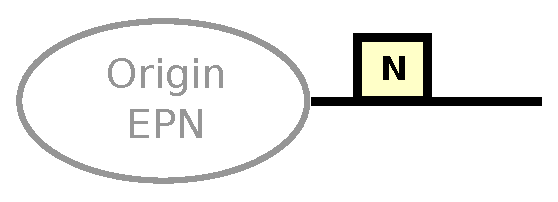
\includegraphics[scale = 0.4]{images/consumption}
  \caption{The \PD glyph for \glyph{consumption}.}
  \label{fig:consumption}
\end{figure}

